\chapter{The straw tracker}\label{chaptertrk}

\textit{The following Chapter will focus on the Mu2e tracker, one of the most important detectors in Mu2e. 
It will give further information about the straw tube tracker panels, 
including the detection mechanism, the mechanical design and the Front End Electronics (FEE).
As previously pointed out, the Mu2e tracker is made up of 216 identical panels. 
Each panel is a mechanical and electrical standalone module. Each panel has 96 drift 
tubes used as fundamental detecting components. I will start by discussing the 
theoretical characteristics of drift tubes and then I will go more in detail with Mu2e tracker features. 
Most of the discussion is based on \cite{kola} and \cite{bobbb}.}

\section{Drift Tubes}
Gas detectors are capable of measuring charged particle coordinates. 
They provide great spatial resolution and detection efficiency at a low cost, Ref. \cite{kola}. 
There are many different gas ionizazion detectors, one of these is the drift tube.
The basic configuration of a drift tube is shown in Figure \ref{fig:drifttube}.
The cylindrical conducting tube, the cathode, is grounded.
A hollow cylindrical conducting tube is grounded and serves as the cathode.
The tube is filled with a combination of noble gas, often Argon, and quench gas. 
A thin sensing wire is suspended along the cylindrical cathode axis. 
The wire, called anode, receives a high voltage. Long and thin drift tubes, known as $straw$ $tubes$, have a similar form.
\begin{figure}[!h]
    \centering
    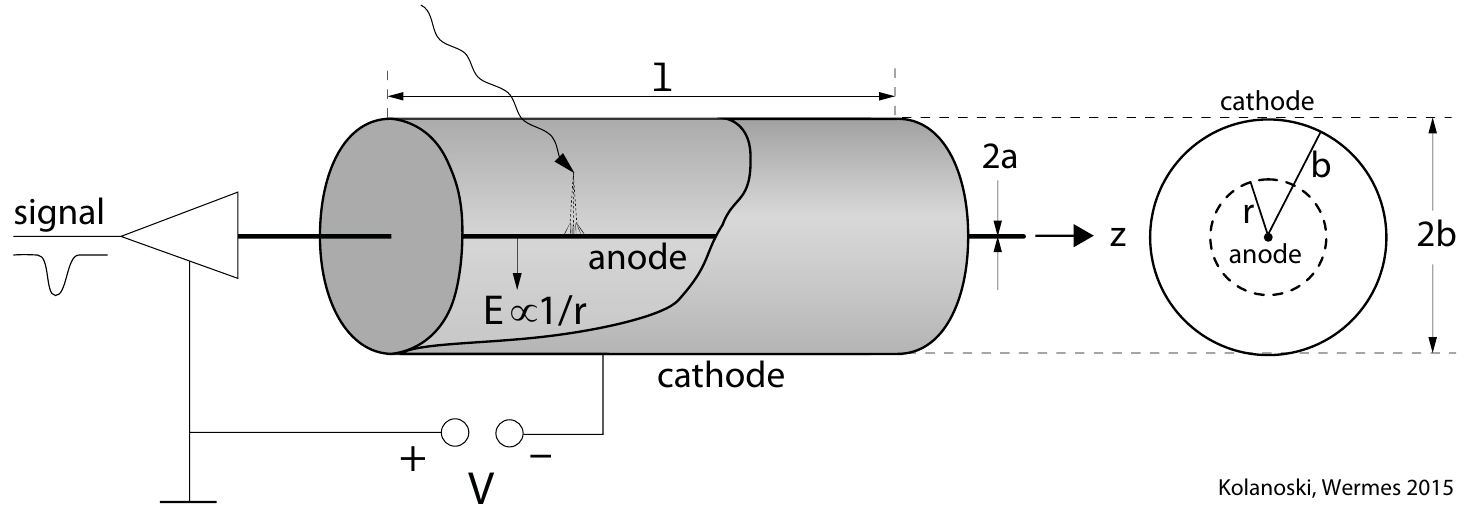
\includegraphics[width =0.8\textwidth]{figures/png/Screenshot_20240324_232621.png}
    \caption{Schematics of a drift tube, Ref. \cite{kola}.}
    \label{fig:drifttube}
    \end{figure}
Assuming an anode radius $a$, a cathode radius $b$ and using Gauss theorem, the electric field is:
\begin{equation}\label{avalanche}
    E(r)=\frac{1}{r}\frac{\lambda}{2\pi \epsilon}=\frac{1}{r}\frac{V}{ \text{ln}(b/a)} \qquad (a<r<b)
\end{equation}
Where $\lambda$ is linear charge density on the wire and $\epsilon$ is the dielectric constant of the gas.
Thinner wires are typically preferred in drift tubes. A greater electric field near the wire increases the amplification factor 
of the drift tube at the same voltage. Additionally, smaller wires improve spatial resolution, Ref. \cite{kola}. 
\subsection{Gas Ionization}
Two are the interactions that can deposit energy when particles traverse the gas volume: ionization and excitation.
Collisions between a charged particle $C$ and an atom $A$ can result in the ejection of one or more electrons: 
$A \ C \rightarrow A^+ e^- C$, or $A \ C \rightarrow A^{++} e^- e^- C$, if more than one electron is released.
This process is called primary ionisation. The mean energy loss per path length can be determined using the Bethe-Bloch formula.
A noble gas atom $A$ can turn also into an excited state $A^*$ through the interaction $A \ C \rightarrow A^* C$. 
If the excitation energy of $A^*$ is higher than the ionization potential of another species $B$ in the gas, the quencher, the
Penning Effect can produce ionization through $A^*B \rightarrow A B^+ e^-$. In addition, the noble gases can
also form molecular ions through processes such as $A^* A \rightarrow A_{2}^{*} \rightarrow A^+_2 e^-$.
A secondary ionisation can occurr through these processes or through electrons that have sufficient energy for generating more ions.
To compute the average number of electron-ion pairs produced by an initial particle, divide its total energy loss 
by the average energy required to make an electron-ion pair. Due to the energy lost during excitation, this average 
does not match the gas ionisation potential. Measurements showed an average of one electron-ion pair every 
30 eV, with variations depending on gas composition and starting particle. Except for very slow particles, 
this value remains constant regardless of their initial energy.
Without an electric field, electrons and ions created during ionisations spread uniformly. 
Collisions cause them to lose energy and eventually reach thermal equilibrium with the surrounding gas. 
They eventually recombine. An electron maximal range during ionisation is correlated with its initial kinetic 
energy. In a normal temperature and pressure gas, a 10 keV electron may be stopped in approximately 1 mm. 
Ionised electrons often have reduced kinetic energy, leading to a shorter range.
\subsection{Drift of Ions and Electrons}
The electric field accelerates free electrons and ions towards the anode and cathode 
along the field lines. As charges accelerate, they scatter on other particles in the gas, 
losing energy. The directions of motion are randomised, and maximum speeds are set. As a result, 
charges move uniformly along the electric field. This is referred to as the drift velocity of the 
charge. It is superimposed with the thermal motions.
Drift velocities for ions and electrons varies based on several parameters. Ions have a bigger mass 
than electrons and their masses are comparable to those of gas molecules. During collisions, gas 
molecules absorb a significant portion of the energy gained from ions during acceleration. In a drift 
tube detector just a little amount of electric field energy enters the energy associated with ion motion, 
making it comparable to the initial thermal energy before acceleration. 
The ion drift velocity $v_i$ is proportional to the reduced electric field $E/N$ where N is the number density of the gas 
and it is typically $\mathcal{O}(10^3)$ cm/ns, except in the region near to the anode wire where a stronger 
electric field is present. The ion thermal velocity is typically $\mathcal{O}(10^4)$ cm/ns at room temperature.
On the opposite, only a small fraction of the energy is released during elastic collision from electrons, 
so they acquire more energy from the electric field than their thermal energy.
Many different factors impact electron drift velocity. Some gas molecules, such as H$_2$O or CO$_2$, 
can interact with electrons to produce negative ions due to their great electron affinity. In rare situations, 
electrons gather enough energy to exceed gas molecule excitation threshold, resulting in inelastic collisions. 
Electron drift velocity is a complex function of electric field intensity due to several variables influencing 
electron collisions across a large energy range. Figure \ref{fig:drift} shows the electron drift
velocity at different electric field strengths in argon-carbon dioxide mixtures (Ar-CO$_2$) of different
proportions, Ref. \cite{ZHAO1994485}.
\begin{figure}[!h]
    \centering
    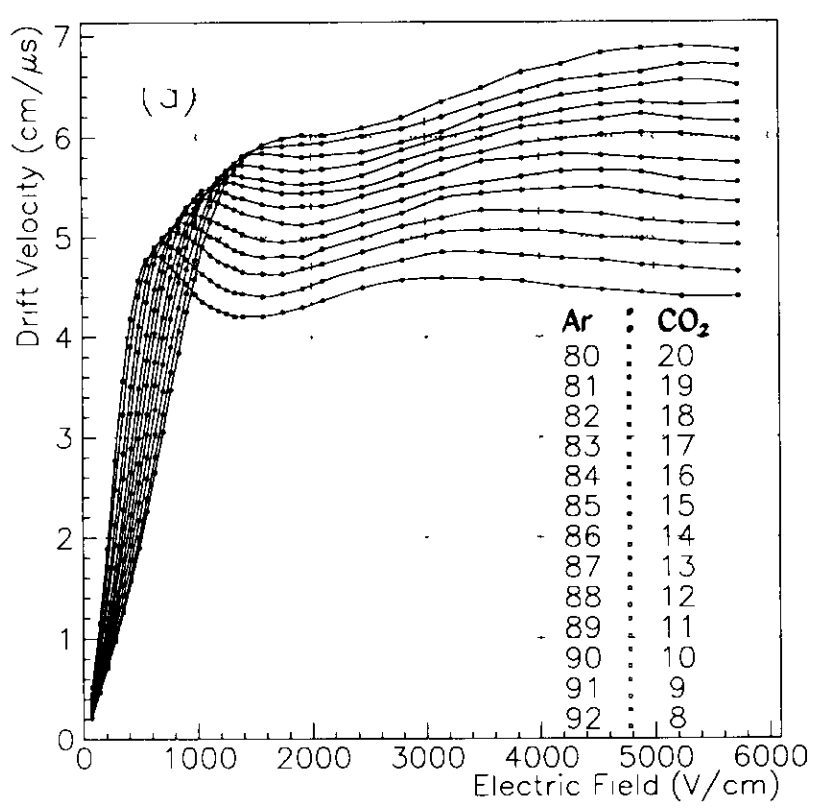
\includegraphics[width =0.7\textwidth]{figures/png/Screenshot_20240330_102206.png}
    \caption{Electron drift velocity versus electric field in Ar:CO$_2$ mixtures of different proportions, Ref. \cite{ZHAO1994485}. 
    80\%:20\% Ar:CO$_2$ mixture is the gas used in the Mu2e tracker.}
    \label{fig:drift}
\end{figure}
Electron drift velocities in drift tubes are typically $\mathcal{O}(10^6)$ cm/ns.
This is significantly higher than ion drift velocities and comparable to electron thermal velocity under the same conditions. 
The radial coordinate of an ionisation can be computed using the electron drift velocity and time.
Since drifting electrons and ions are scattered on gas molecules, they also diffuse along their trajectory. 
Electrons diffuse significantly quicker than ions because of their high velocity. Electron diffusion limits 
the intrinsic resolution of drift tubes used to measure incoming particle coordinates. CO$_2$ has internal 
degrees of freedom at low collision energies, preventing electron energies from exceeding thermal energy until 
field strengths above about 2 kV/cm. This improves intrinsic spatial resolution.
\subsection{Avalanche Multiplication}
Electrons can ionise when they face a high electric field near the anode wire. 
The released secondary electrons form tertiary electrons, and so on. Free electrons rapidly multiply, 
resulting in an avalanche. In a drift tubes, where the electron mean free path is about the order of $\mu$m, 
an avalanche develops when the electric field approaches $\mathcal{O}(10)$ kV/cm. 
According to Equation \ref{avalanche}, using $a \sim \mathcal{O}(10^{-3})$ cm, $b \sim \mathcal{O}(1)$ cm and
a normal voltage of 1-2 kV, the avalanches can occur within $\mathcal{O}(100) \ \mu$m from the anode wire. 
Electrons from the avalanche are collected on the anode wire within 1 ns, while positively charged ions move towards the cathode.
Drifting ions mostly generate signals in electrodes via induction. Figure \ref{fig:avalanche} shows the model of an ionisation avalanche.
\begin{figure}[!h]
    \centering
    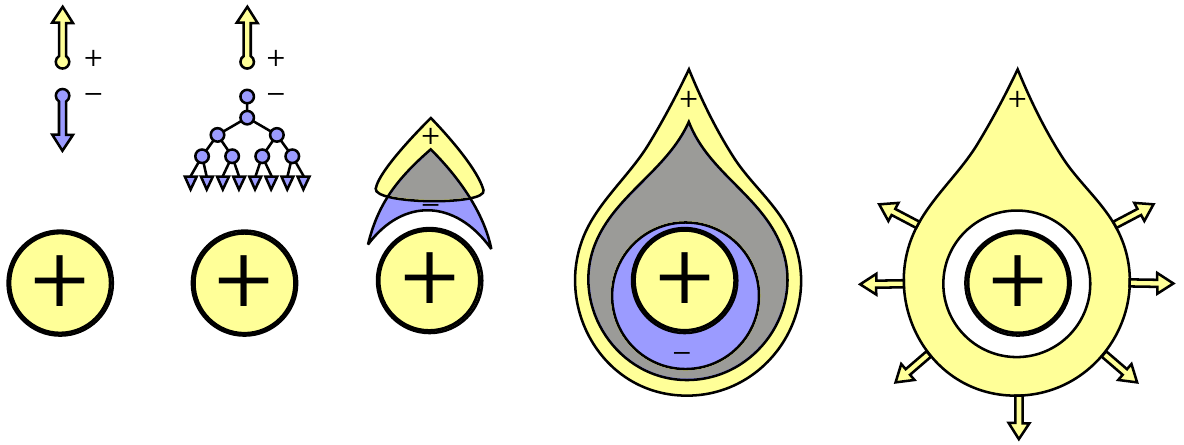
\includegraphics[width =0.7\textwidth]{figures/png/Screenshot_20240330_182509.png}
    \caption{The model of an ionisation avalanche forming at the anode wire of a proportional tube or chamber, Ref. \cite{kola}. 
    (a) In the drift volume, electrons and ions are generated and drift to their corresponding electrodes. 
    (b) Near the wire, the electron achieves a high enough field to induce secondary ionisation, resulting in an avalanche. 
    (c) The electric field separates charges created during an avalanche. 
    (d) Electrons have higher lateral diffusion than ions, causing the avalanche to expand 
    around the wire and produce a positive charge cloud in the shape of a drop. 
    (e) Electrons from the avalanche reach the anode within nanoseconds, but ions take longer, up to ms, to reach the cathode.}
    \label{fig:avalanche}
\end{figure}
\subsubsection{Avalanche Gain}
When an avalanche develops, the amplification factor is around $10^4-10^6$. The number of electrons freed per unit path length is given
by the first Townsend ionization coefficient $\alpha=\sigma_{ion}n=1/\lambda_{ion}$ and this depends on the electric field $E$, 
as a higher electric field corresponds to a higher kinetic energy of the electron, that increases the ionization cross-section.
The increase $dN$ of the number of electron-ion pairs over a path length $ds$ is, Ref. \cite{kola}:
\begin{equation}
    dN=\alpha(E)Nds
\end{equation}
Solving this equation, we can easily obtain the gas amplification $G$:
\begin{equation}\label{av}
    G=\frac{N(s_a)}{N_0}=\text{exp} \left( \int_{s_0}^{s_a} \alpha(E(s)) ds \right)=\text{exp} \left( \int_{E_{min}}^{E(a)} \frac{\alpha(E(s))}{dE/ds} dE \right)
\end{equation}
where $N_0$ corresponds to unamplified electrons in $s=s_0$ and $E_{min}$ corresponds to the minimum energy 
for ionisation to occurr. The energy distribution depends on the electric field which is position dependent. 
Since the free path is inversely proportional to the particle density in the gas, $E_{min}(\rho)=E_{min}(\rho_0)\rho/\rho_0$.
It is reasonable to say that the coefficient is proportional to the field strength, $\alpha= \beta E$, in the low field region. 
Adding this relation with Equation \ref{avalanche} and \ref{av}:
\begin{equation}
     \text{ln}(G)=\beta \ a \ E(a) \ \text{ln}\left( \frac{E(a)}{E_{min}}\right)
\end{equation}
where $\beta$ can be related to $w_i$, that is the energy spent for one ionisation and its value is equal to $e \Delta V$.
As the voltage drop per unit path length is $dV = E(s)ds = (\alpha/\beta)ds$, we obtain $dN=N \beta dV$. Integrating, we can see that
$\beta= \text{ln}(2)/\Delta V$, so the gain in a drift tube is:
\begin{equation}
     \text{ln}(G)=\frac{ \text{ln}(2)}{\Delta V} \ a \ E(a)  \ \text{ln}\left( \frac{E(a)\rho_0}{E_{min}(\rho_0)\rho}\right) \qquad E(a)=\frac{V}{a ln(b/a)}
\end{equation}
which is the Diethorn's formula. 
Gain measurements with variable $\rho$/$\rho_0$, $a$, and $E(a)$ can provide the parameters $E_{min} (\rho_0)$ and $\Delta V$. 
The gas temperature $T$, pressure $P$ and operating voltage $V$ significantly impact the gain of a drift tube with a particular shape and gas mixture. 
\subsubsection{Quench Gas}
To avoid subsequent avalanches, the drift tube gas combination may contain a quench gas, such as CO$_2$, 
methane, or other hydrocarbons. During an avalanche, photons are created by gas deexcitation and electron 
attachment to electronegative species, resulting in negative ions. Photons can generate ionisations 
outside the primary avalanche zone or create free electrons on the cathode surface, resulting in secondary avalanches.
The difficulty arises when the signal created is not proportional to the deposited energy by the original particle 
and is no longer localised to the energy deposition point. Enough intense photons can induce a chain reaction of 
secondary avalanches, leading to a continuous discharge. The use of quench gas prevents subsequent 
avalanches by absorbing ionising photons before they travel far. A tiny quantity of quench gas during normal operation 
can significantly decrease secondary avalanches and breakdowns.
\subsubsection{Operation Modes of Gaseous Ionization Detectors}
In drift tube detectors, the number of electron-ion pairs formed during an avalanche is 
proportional to the starting number of electrons, as shown in the gain computation. To 
operate in a proportional mode, an appropriate voltage is needed to reduce the effects 
of avalanche charges on the electric field. Figure \ref{fig:gaseous} illustrates how a 
gaseous ionisation detector may work in multiple modes based on the operating voltage. Higher operating 
voltage leads to higher charges on the electrodes. Low voltage causes ionisation charges to recombine 
before reaching electrodes, leading to no signal collection. At higher voltages, in ionisation chamber 
region, charges can drift to electrodes, but the electric field is insufficient for avalanches to occur. 
Increasing the operational voltage leads to drift tubes and proportional counters. When the voltage 
becomes high enough, proportionality is lost. When electrons from an avalanche are collected, 
the high density of positive ions near the anode might affect the electric field. 
Electrons in future avalanches that enter the area between the positive ion cloud and the wire face a 
decreased electric field, resulting in lower amplification. The electric field becomes greater in the 
tail of the avalanche, which is far from the wire than the ion cloud. This range of voltage is called region of 
limited proportionality. When the operating voltage reaches high values, 
avalanches create sufficiently energy photons to cause secondary avalanches 
that propagate across the detector, independently from the quench gas. 
This results in detector saturating the output. This way of operating is 
called breakdown mode, commonly known as the Geiger-Muller mode.
\begin{figure}[!h]
    \centering
    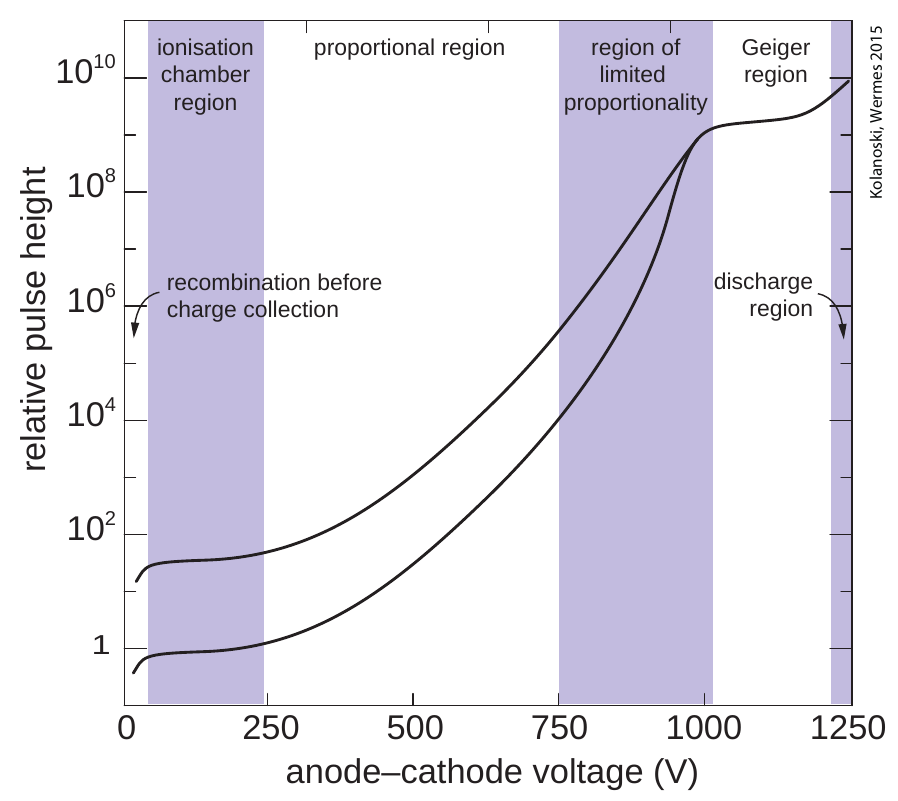
\includegraphics[width =0.5\textwidth]{figures/png/Screenshot_20240330_203416.png}
    \caption{The dependence of particle gain on applied voltage in gaseous ionisation detectors. 
    The numbers on the axes are for orders of magnitude only and they depend on the device geometry and gas concentration. 
    Drift tubes operate in the proportional mode, Ref. \cite{kola}.}
    \label{fig:gaseous}
    \end{figure}
\subsection{Signal Creation and Propagation}
Drift tube signals do not originate from avalanche charges. In this case, the anode wire would 
receive the complete signal within a few ns. Signal pulses are created by charges on electrodes 
caused by electron and ion mobility. The Shockley-Ramo theorem, Ref. \cite{kola}, can be 
used to determine the induced charge and current. 
The Shockley-Ramo theorem yields various important results. The total induced charge of a moving charge 
$q$ is determined by the initial and final positions only.  A charge pair induces the same amount of 
charge on an electrode as the charge collected on it. Furthermore, if all electrodes are treated as 
an unity, their weighted potential will be one. 
If one electrode completely encloses the others, the weighted field in the contained region is always zero. 
This means that the total induced current across all electrodes is always zero. The Shockley-Ramo theorem can 
be applied to the drift tube. In an avalanche with $N$ electron-ion pairs, we evaluate the induced current 
signal on the anode wire. The current on the cathode has an additional negative sign. The weighted 
potential and field in the straw depend on the radial coordinate $r$:
\begin{equation}
    \psi_w(r)=\frac{\text{ln}(b/r)}{\text{ln}(b/a)}
\end{equation}
\begin{equation}
    \textbf{E}_w(r)=\frac{1}{\text{ln}(b/a)}\hat{\textbf{r}}
\end{equation}
As previously mentioned, the drift velocity of ions, $u$, is proportional to the electric field intensity $E$. Therefore, $u$ = $mu \ E$. 
Then the ion trajectory fulfils:
\begin{equation}
    u=\frac{dr(t)}{dt}=\frac{\mu V_0}{r(t)\text{ln}(b/a)}
\end{equation}
When ionisation occurs at the anode, the starting condition can be approximated as $r(0) = a$. So, the solution to the given differential equation is:
 \begin{equation}
    r(t)=a \sqrt{1+\frac{t}{t_0}} \qquad t_0=\frac{a^2 \ln (b / a)}{2 \mu V_0}
    \end{equation}
Here, $t_0$ represents the characteristic time, which is generally on the order of 1 ns. 
The time $t$ falls within the range $0 < t < t_{max}$, where $t_{max} = t_0 [(b/a)^2 - 1]$. 
The induced current and charge from the wire are expressed as:
 \begin{equation}
    I_{i o n}^{i n d}(t)=-(e N) E_w(r) \frac{\mathrm{d} r(t)}{\mathrm{d} t}=-\frac{e N}{2 \ln (b / a)} \frac{1}{t+t_0}
    \end{equation}
    \begin{equation}
        Q_{\text {ion }}^{\text {ind }}(t)=\int_0^t I^{\text {ind }}\left(t^{\prime}\right) \mathrm{d} t^{\prime}=-\frac{e N}{2 \ln (b / a)} \ln \left(1+\frac{t}{t_0}\right)
        \end{equation}
The total charge created on the wire by the travelling electrons is:
\begin{equation}
    Q_e^{i n d}=-e N\left[\psi_w(a)-\psi_w\left(r_{a v g}\right)\right]=-e N \frac{\ln \left(r_{a v g} / a\right)}{\ln (b / a)}
    \end{equation}
    where $r_{avg}$ is the average position of ionisations in the avalanche. When compared to the total charge 
    induced $Q^{ind}_{tot}(t_{max}) = -eN$, electron mobility in the avalanche accounts for just 1-2\%. 
    Positive ion drift from the avalanche accounts for the majority of the signal. A signal propagates 
    to both ends of the drift tube from the avalanche location.
    Signals with distinct frequency components can propagate at varying velocities. This causes the signal to disperse.
    When determining the longitudinal coordinate of an avalanche using the signal arrival time difference between straw tube ends, various complications emerge.
%For low-frequency components of the signal (for a meter-long drift tube, this translates to a frequency much less than 300 MHz), 
%a quasi-electrostatic approach is sufficient. The signals seen at tubes ends are influenced by impedances between and on the electrodes. 
%On the other hand, for the high-frequency components of the signal, the tube needs to be treated as a transmission line. 
%The propagation speed of a signal wave with frequency $\omega$ is then $c/\sqrt{\omega}$ $\epsilon$($\omega$), 
%where $c$ is the speed of light and $\epsilon$ is the dielectric constant of the gas. As $\epsilon$ is a function of $\omega$, 
%components of different frequencies propagate at slightly different velocities. This leads to a dispersion (widening) of the signal. It brings some subtleties when using signal arrival time difference between straw tube ends to determine the longitudinal coordinate of an avalanche.
\section{The tracker panels}
The Mu2e tracker straw tube arrays use the same detection principles as the gaseous ionisation detectors, Ref. \cite{kola}, 
but it has a significant different design and manufacturing improvements to meet the experiment precise requirements.
\begin{figure}[!h]
    \centering
    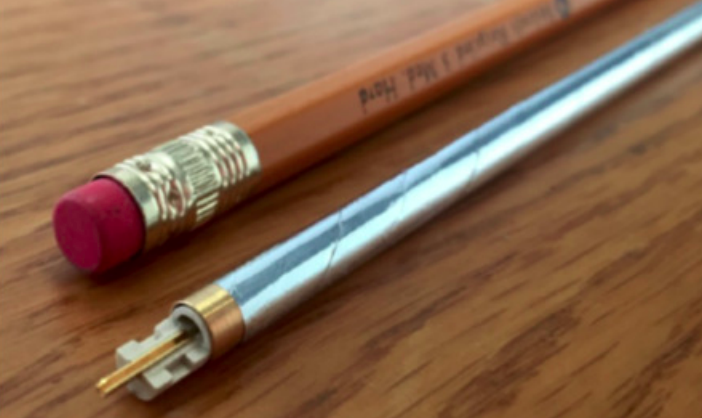
\includegraphics[width =0.5\textwidth]{figures/png/Screenshot_20240327_000000.png}
    \caption{A picture of the Mu2e straw tube
    compared to a pencil, Ref. \cite{trk}.}
    \label{fig:trkpencil}
    \end{figure}
    \begin{figure}[!h]
        \centering
        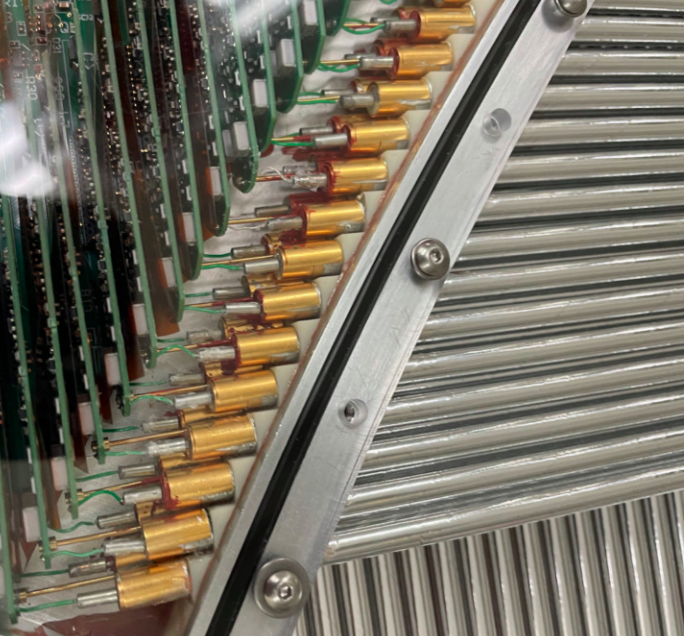
\includegraphics[width =0.5\textwidth]{figures/png/Screenshot_20240327_000131.png}
        \caption{The fully assembled tracker panel with its straws, Ref. \cite{trk}.}
        \label{fig:strawtubes}
        \end{figure}
The straw tubes used in the Mu2e tracker \ref{fig:trkpencil} are 5 mm in diameter and 0.33 - 1.17 m in length, 
Ref. \cite{bartoszek2015mu2e}. The straws are wound with two layers of 6 $\mu$m-thick metallized Mylar and a 3 
$\mu$m layer of glue in between. The straw wall is 15 $\mu$m thick: this helps to minimize the amount of materials 
in the tracker, lowering the total energy loss from the observed electrons. Furthermore, it minimises the likelihood 
of significant deflections in electron trajectories, facilitating track reconstruction. As a result, the experiment 
will have a very good momentum resolution. The straw tube anodes are composed of gold-plated tungsten wires 
with a diameter of 25 $\mu$m. The straws and anode wires are tensioned and work-hardened to avoid sagging.
\begin{figure}[!h]
    \centering
    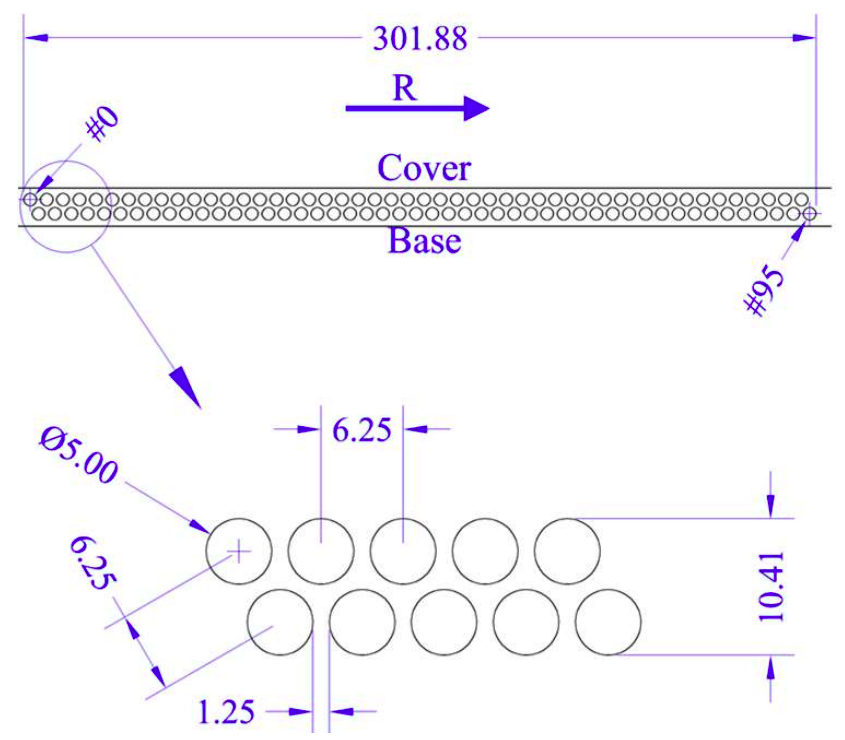
\includegraphics[width =0.6\textwidth]{figures/png/Screenshot_20240326_234405.png}
    \caption{Straw arrangement in a tracker panel, Ref. \cite{trk}.}
    \label{fig:trktubes}
    \end{figure}
To create a perfect electric field with adequate spatial resolutions, the anode wires are oriented 
to the panels with a precision of at least 25 $mu$m in the radial direction and 50 $mu$m in the 
perpendicular direction. All panels are x-ray scanned to accurately measure and document the wire 
locations of straw tube channels. Figure \ref{fig:trkpencil} shows the 
termination mechanism that holds the wire in place.
To increase mechanical strength, a brass tube is joined to either end of the straw using silver epoxied, Ref. \cite{bartoszek2015mu2e}. 
To ensure electrical isolation, a Kapton sleeve is put within the brass tube. An injection-molded plastic insert is then connected 
inside the sleeve. The insert contains a semicylindrical duct that allows gas to enter and exit the straw tube. The insert 
has a groove along its axis and a U-shaped brass anode pin inserted at the end. To avoid slippage, the anode wire is 
epoxied into the groove and soldered to the anode pin.
A T-shaped pin protector protects the anode pin from breaking by covering the groove in the plastic insert. 
The pin protector is epoxied to the insert, with an extra brass ring connecting them. A ground clip 
is silver-epoxied to two adjacent straws on the brass tubes and rings, providing a shared ground connection 
for the straws. 
Signals are sent to a common pre-amplifier (preamp) board via the anode pin pair and grounding clip. 
The FEE will be introduced later. Figure \ref{fig:strawtubes} shows completely built straws in a tracker panel. 
Each panel has 96 straw tubes organised in two staggered layers for improved tracking. Figure \ref{fig:trktubes} 
show the detailed spatial arrangement of the straws, Ref. \cite{trk}. Channels are numbered from 0 (longest) 
to 95 (shortest), starting with the radially innermost straw.
Straws are spaced by 1.25 mm and can expand under gas pressure, Ref. \cite{bartoszek2015mu2e}.
The Mu2e tracker panels uses a gas flow of 80\%:20\% Ar:CO$_2$. 
The vacuum environment within the Detector Solenoid reduces the impact of electron scattering on trajectories. 
However, the tracker panels, particularly the straws, must endure pressure differences. Under normal temperature 
and pressure, each panel must have an average leak rate of 0.014 cm$^3$/min. The nominal operating voltage of 
the straw tube channels is 1450 V. An earlier investigation on a prototype of the tracker showed the straw tube 
gain as 1.25 $\times$10$^4$ at 1250 V and 7 $\times$ 10$^4$at 1425 V. According to Diethorn's calculation, Equation \ref{XXX}, 
the gas gain at 1450 V is around 1 $\times$10$^5$.

\section{The tracker Front-End Electronics}
Before being accessible to the Mu2e Data Acquisition (DAQ) system, the analog signals 
from the tracker straw tube channels need amplification, digitization and packaging. 
The tracker front-end electronics (FEEs) are designed to achieve these goals. The FEEs 
consist of multiple Printed Circuit Boards (PCBs) as shown in Figure \ref{fig:trackerfee}, Ref. \cite{vadimmu2e}.
All PCBs are situated in the outer section of the panel. Pulse timing is measured at the 
end of each straw, in order to be able to measure electron position on the wire. A measure 
of $dE/dx$ is provided, so pattern recognition can be possible, Ref. \cite{bartoszek2015mu2e}. For this purpose each straw has:
\begin{itemize}
    \item two preamp channels, one for each end;
    \item two TDC channels, one for each end;
    \item one ADC channel, measuring sum of both ends;
    \item one High Voltage feed.
\end{itemize}
There are 46,080 preamps and TDCs and 23,040 ADC channels. There are two sides of the panel, one called HV side and one called CAL side. 
\begin{figure}[!h]
\centering
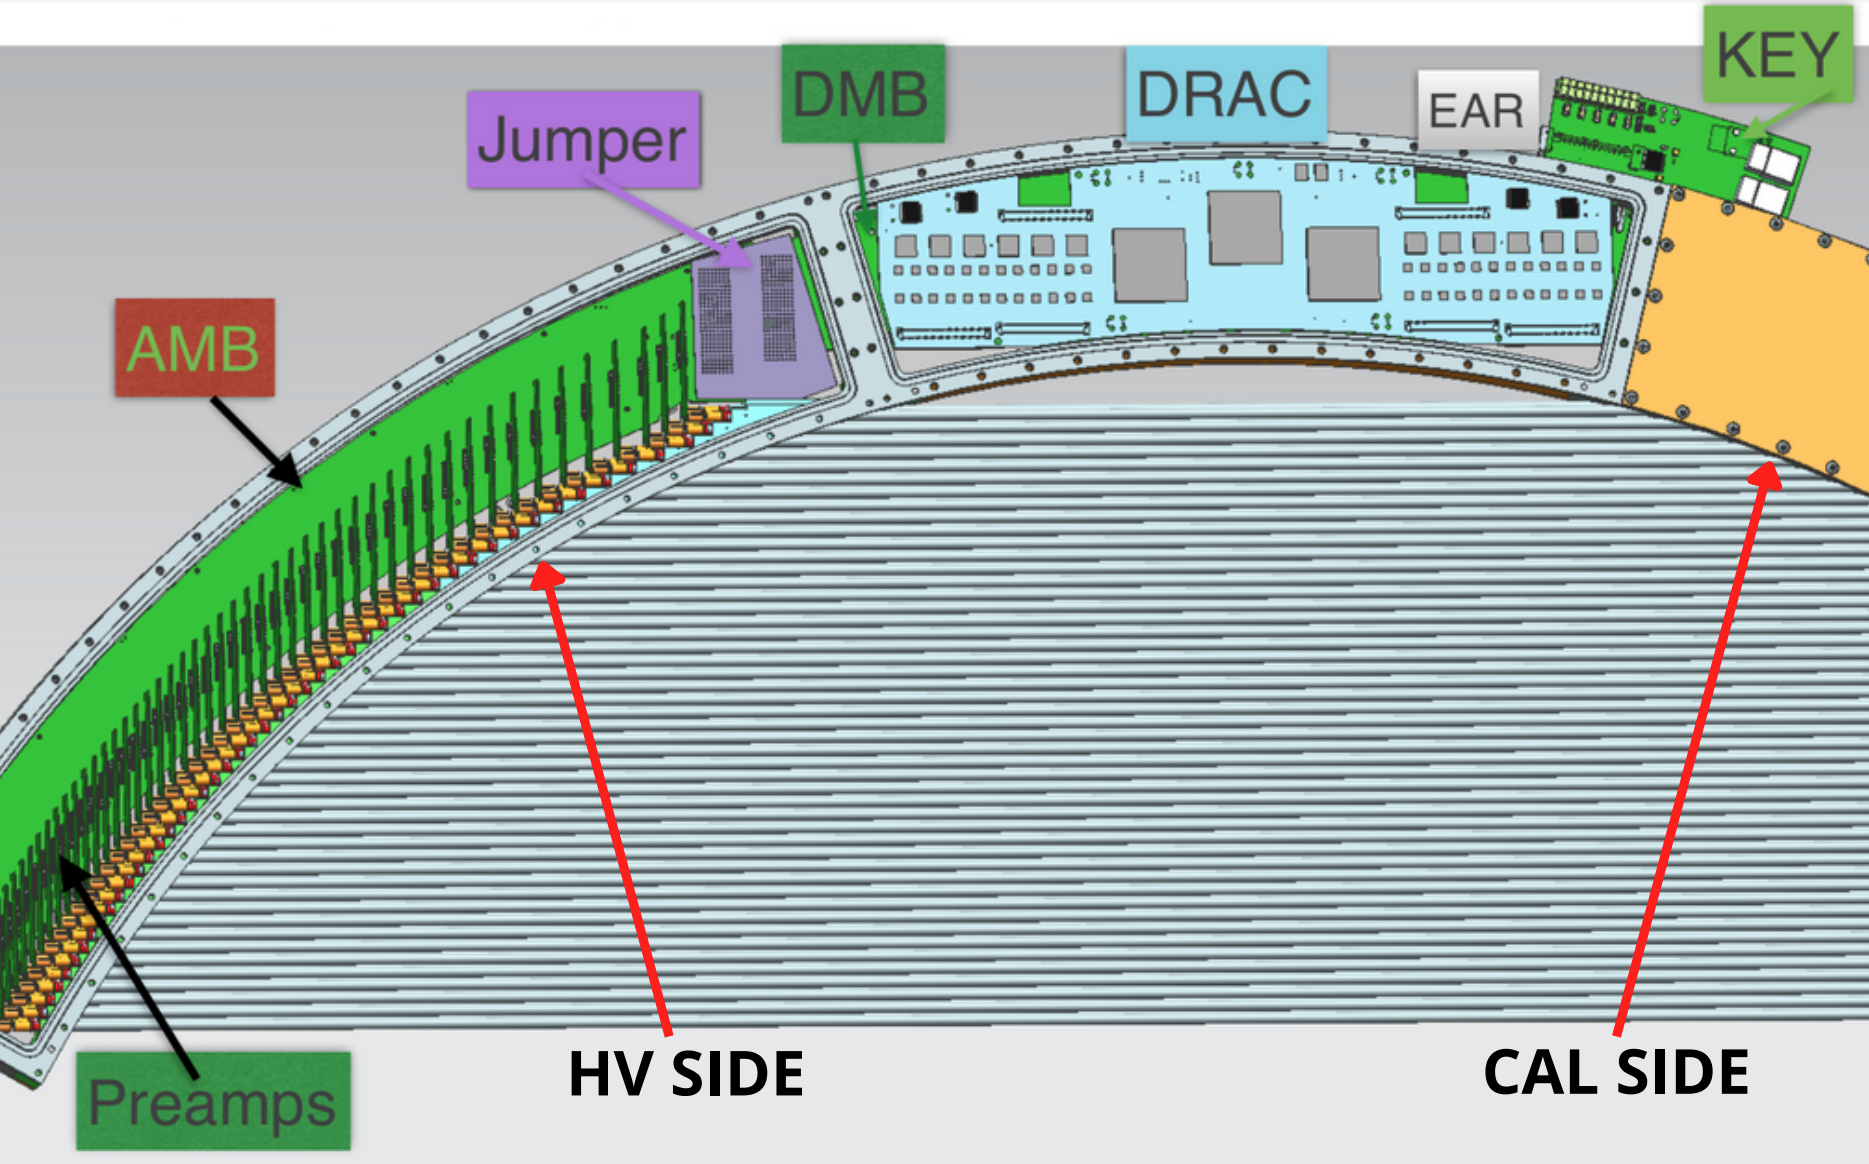
\includegraphics[width =0.8\textwidth]{figures/png/Screenshot_20240131_111836.png}
\caption{An overview of the tracker front-end electronics (FEE), Ref.  
\cite{vadimmu2e}. The preamps and the Analog Motherboard (AMB) 
on the other side of the straws are not shown in the figure.}
\label{fig:trackerfee}
\end{figure}
On either side, there are an Analog Mother Board (AMB) and a Jumper board, 
which task consist of directing signals from the preamps towards the Digital 
Motherboard (DMB) positioned at the center, then to the Digitizer Readout and 
Assembler Controller (DRAC) (mounted on top of the DMB) to be processed and 
temporarily stored. Both the AMBs and the DMB handle low voltage distribution 
and the HV side of the AMB distributes high voltage to the straw anode wires, 
reason why it is called this way. On the AMBs and the DMB there are sensors, 
monitoring environmental variables such as temperature, pressure and humidity. 
The low voltage power supply is fed into the panel through the KEY. The KEY 
contains an optical fiber link and a JTAG interface for communication. The 
frontends components were chosen to sustain high level of radiation.
\subsection{Pre-Amplifiers}
The pre-amplifiers (preamps) are responsible for the initial readout of 
signals from both ends of the straw tube channels. As previously explained, 
the channels are read out from both ends and two adjacent channels are linked 
to the same preamp. Each tracker panel contains 48 preamps on the HV side, 
while an additional 48 preamps are located on the opposite side, the CAL one. 
Preamps are mounted vertically on the AMBs. Preamps are required to have a 
matching 300 $\Omega$ input impedance with the straw, in order to avoid signal 
reflections. The preamps convert the straw tube current signals into voltage signals. 
Signals are amplified and shaped. The preamps on the CAL and HV sides aren't 
exactly the same. The CAL preamps have circuitry that can inject calibration 
pulses into the channel. This capability enables the channel readout electronics 
to be tested without a high voltage source. The preamps on the HV side distribute 
the high voltage supply to individual straw tubes. 
%The voltage gains of individual channels, different from the gas gain, are set by control signal from the DRAC. A bias voltage, adjustable for each side of a channel, is applied to the signals. 
\subsection{Digitizer Readout and Assembler Controller}\label{DRAC}
The brain of a tracker panel is called Digitizer Readout and Assembler Controller (DRAC). 
The DRAC is responsible for digitizing, packaging and temporary storage. It also controls 
panel operations. The schematics of the DRAC board is shown in Figure \ref{fig:drac}. In 
this figure Analog to Digital Converters (ADCs), DDR3 memories and compators are shown. 
The large chips in the centers are the Field-Programmable Gate Arrays (FPGAs). The one 
in the center is the Readout Controller (ROC), which manages communications, monitors 
slow control variables and controls panel operations \ref{ROC}. The left and the right 
ones, which are referred to as the digi FPGAs, are responsible for monitoring data output, 
buffering data and assembling data packages. Each of them refers to 48 straw channels. 
\begin{figure}[!h]
\centering
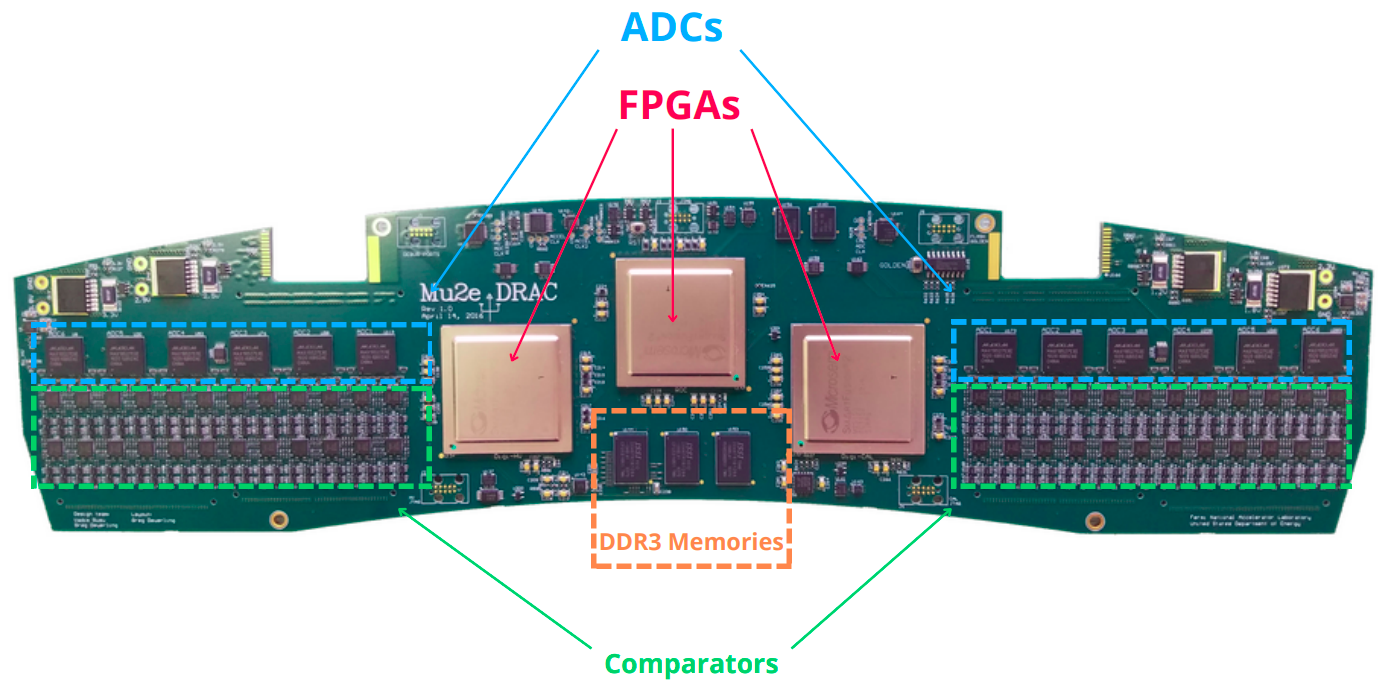
\includegraphics[width =\textwidth]{figures/png/Screenshot_20240204_115052.png}
\caption{Digitizer Readout and Assembler Controller (DRAC) board schematics, Ref. \cite{drac}. 
The DRAC board is the brain of the tracker panel. In this figure Analog to Digital Converters (ADCs), FPGAs, DDR3 memories and compators are shown.}
\label{fig:drac}
\end{figure}
In figure \ref{fig:flowfee}, signal flow in the tracker FEEs is reported. At the 
beginning the signal coming from both ends of the straw is routed to the preamps. 
After that, the analog signal is sent through the microstrip transmission line to 
the digitizers. In the DRAC, the two biased signals are fed independently to 
zero-crossing comparators, which produce square pulses when the signals exceed 
their respective thresholds. The squared pulses are sent to Time-to-Digital Converters 
(TDCs, firmware based, 16 bits each) implemented in the digi FPGAs, that have the task 
of digitizing the trigger timings, including the arrival time and the time over threshold, 
at a rate of about 62.5 MHz. Besides drift time, TDCs measure time difference across the 
straw to estimate position along the wire and the intrinsic time resolution of TDC is about 
25 ps, adding comparator jitter, noise and other external effects the final resolution is 
$\sim$ 70 ps for time division. Furthermore, an integrator adds voltage signals coming 
from the two straw ends. In data collection, a hit occurs when both ends of a straw channel 
are simultaneously activated. The total is digitized by a 12-bit (10-bit ENOB) ADC at 40 MHz
and then sent to the digi FPGA. The digi FPGA creates a data packet for each hit based on 
TDC and ADC information. This suppresses false triggers caused by random electrical noise. 
The Digitizer receives signals from both ends of four straws and multiplexes them into one 
output buffer before sending a packet of data to the ROC. Signals are sent to the ROC at 
200 MHz. The data packets are then briefly stored in DDR3 memory for further use by the 
DAQ system. It is important to save also the voltage signal, since the pulse height 
information can help us to reject proton background, a significant source of noise 
or to distinguish muons from electrons. The proton signal will appear as a saturated flag, 
since the proton $dE/dx$ is $\times$50 the electron one.
\begin{figure}[!h]
\centering
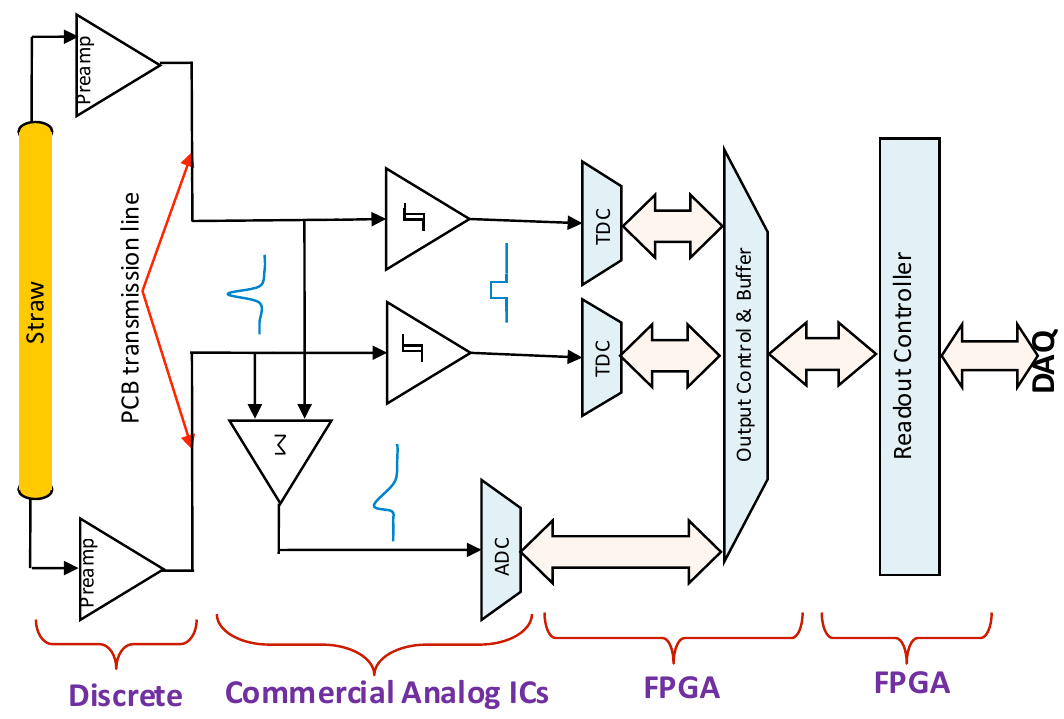
\includegraphics[width =0.8\textwidth]{figures/png/Screenshot_20240203_135048.png}
\caption{Signal flow through front end electronics, Ref. \cite{bartoszek2015mu2e}.}
\label{fig:flowfee}
\end{figure}

\subsection{Read-Out Controller}\label{ROC} 
The main job of the ROCs (one per panel, 216 in total) 
is to collect data from the digitizer boards, buffer data and 
send them to DAQ. They are based on an FPGA architecture. They 
continuously stream out the zero-suppressed data collected between 
two proton pulses from the detectors, in this case the tracker, to 
the Data Transfer Controllers (DTCs), Ref. \cite{GIOIOSA2023167732}. The buffer 
stage is fundamental, since during the beam inter-spill time (836 ms 
out of each 1333 ms), we want us to be able to take data from cosmic 
rays, even if the rate will be very low. For this purpose, the ROCs 
include external DRAM. The communication is flexible, thanks to the 
programmable nature of digitizer, ROC and DAQ. 
\section{Requirements on tracker Performance}
Here a resume of the requirements that the tracker must satisfy to ensure the success of the experiment is presented, Ref. \cite{trkreq}.
A momentum resolution less than 180 keV/c for a 105 MeV/c electron is needed in the nominal
1 Tesla solenoidal field, as measured at the front face of the tracker volume (before
passing through any tracker related material). Non-Gaussian tails, particularly any
high-side tail, must be controlled such that the DIO background results in much less
than one event at design sensitivity. To reach this, simulation results indicate that 
a single straw requires around 4 cm of longitudinal and 200 $\mu$m of transverse resolution for drift path lengths. 
It must have an acceptance of approximately 20\% for conversion electrons.
The tracker must operate in an ambient vacuum (< $10^{-4}$ Torr).
It should be able to withstand a rate of 5 MHz per straw (highest rate straw) 500 ns after the spill. This is
for background studies. The nominal experiment live time starts 700 ns after the spill.
